\documentclass{beamer}
\usetheme{metropolis}
\title{Antarctic Ice Shelves and Ice Sheets near the Surface}
\date{\today}
\author{J. C. Hanson (CCAPP, The Ohio State University)}
\institute{CCAPP @ OSU}
\usepackage{outlines}
\usepackage{enumitem}
\usepackage{graphicx}
\usepackage{amsmath}
\setenumerate[1]{label=\Roman*.}
\setenumerate[2]{label=\Alph*.}
\setenumerate[3]{label=\roman*.}
\setenumerate[4]{label=\alph*.}
\newcommand{\sign}{\text{sgn}}
\usepackage{siunitx}

\begin{document} \maketitle
\small

\begin{frame}{Ten Minute Talk on Ice Shelves and Ice Sheets Near Surface}
\begin{outline}[enumerate]
\1 Dr. Connolly has returned from Weizmann Institute with good news
\1 Part of those discussions require a review of knowledge for ice studies
\2 Emphasis on firn properties
\2 Emphasis on (possible) surface waves
\1 Physics of an ice column
\1 The Landau-Lifshitz/Looyenga equation
\1 Review of Results from Moore's Bay (2011-12)
\1 Review of Results from ARA Analyses (2011-present)
\end{outline}
\end{frame}

\begin{frame}{Ten Minute Talk on Ice Shelves and Ice Sheets Near Surface}
ARIANNA/ARA have a few key differences, that inform how the projects can be combined
\begin{columns}[T]
\begin{column}{0.6\textwidth}
\centering
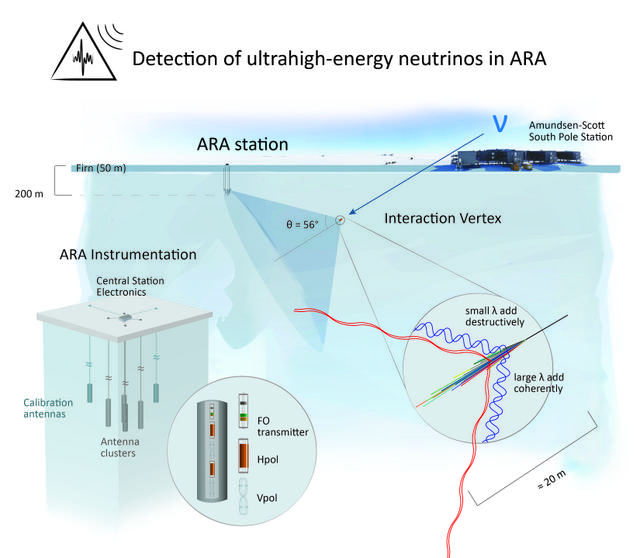
\includegraphics[width=\textwidth]{ara_overview.png}
\end{column}
\begin{column}{0.4\textwidth}
\centering
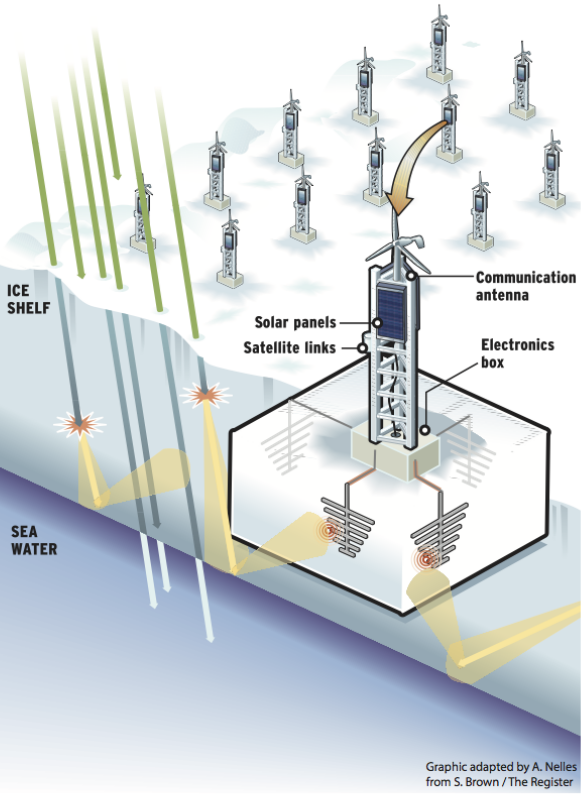
\includegraphics[width=\textwidth]{arianna_overview.png}
\end{column}
\end{columns}
\end{frame}

\begin{frame}{Ten Minute Talk on Ice Shelves and Ice Sheets Near Surface}
\begin{outline}[enumerate]
\1 Why do we believe that the firn density profile is exponential? 
\1 Why do we believe index of refraction tracks density?
\end{outline}
\end{frame}

\begin{frame}{Theoretical Exponential Density Requirements}
Let the firn be represented by $N$ discrete blocks of firn labelled by $j$, each with a volume $A\Delta z$, and a density $\rho_j$.  A height of $0$ m corresponds to the first block ($j=0$) at the bottom of the stack, and the height of the stack is $h = N \Delta z$.  The force down on block $j$ is balanced by a normal force:
\begin{equation}
F_j = \rho_j v_j g + \sum_{i=j+1}^N \rho_i v_i g
\end{equation}
The force down on block $j+1$ is balanced by a normal force:
\begin{equation}
F_{j+1} = \rho_{j+1} v_{j+1} g + \sum_{i=j+2}^N \rho_i v_i g
\end{equation}
\end{frame}

\begin{frame}{Theoretical Exponential Density Requirements}
\textbf{Using $v_{j} = v_{+1} = A\Delta z$}, we have
\begin{equation}
\frac{F_{j+1}-F_{j}}{gA\Delta z^2} = \frac{\rho_{j+1}-\rho_{j}}{\Delta z} + \frac{1}{\Delta z^2}\left(\Delta z\sum_{i=j+2}^N\rho_i - \Delta z\sum_{i=j+1}^N\rho_i \right)
\end{equation}
Letting $\Delta z \rightarrow 0$, and $z_0 \leftrightarrow j$, $z_1 \leftrightarrow j+1$, we have
\begin{equation}
\frac{F'}{gv} = \rho'(z) + \frac{1}{dz^2}\left(\int_{z_1}^h \rho(z)dz + \int_{z_0}^{h}\rho dz \right)
\end{equation}
We can also combine the integrals by reversing one, and eliminating $h$.
\end{frame}

\begin{frame}{Theoretical Exponential Density Requirements}
This leaves
\begin{equation}
\frac{F'}{gv} = \rho'(z) + \frac{1}{dz^2}\left(\int_{z_0}^{z_1} \rho(z)dz \right)
\end{equation}
The derivative of the normal force approaches zero as fast as the volume element.  \textbf{Thus, the left side is a constant.}  Taking the derivative with respect to $z$ of both sides, and rearranging:
\begin{equation}
0 = \rho''(z) + \frac{\rho(z_1)-\rho(z_0)}{dz^2}
\end{equation}
Recall that $v/dz = A$.  Multiplying both sides by $v$ and rearranging yields:
\begin{equation}
\rho''(z) = -\left(\frac{A}{v}\right)\frac{\rho(z_1)-\rho(z_0)}{dz} = -\left(\frac{A}{v}\right) \rho'(z)
\end{equation}
\end{frame}

\begin{frame}{Theoretical Exponential Density Requirements}
Finally:
\begin{equation}
\rho''(z) = -\left(\frac{A}{v}\right) \rho'(z)
\end{equation}
which has the solution ($A/v \equiv z_0^{-1}$):
\begin{equation}
\boxed{\rho(z) = R_0 \exp(-z/z_0) + \rho_0}
\end{equation}
In this coordinate system, up is positive, $z = 0$ corresponds to the highest density, and $z = h$ is the surface.  (The assumptions are not always valid, so be careful).  The two remaining constants are derived from the snow density and the bulk ice density.
\end{frame}

\begin{frame}{Landau-Lifshitz/Looyenga Equation}
For a material comprised of a mixture of two dielectrics, the complex dielectric constant is:
\begin{equation}
\epsilon_{mix} = \left(v_1\epsilon_1^{1/3} + v_2\epsilon_2^{1/3}\right)^3
\end{equation}
The constants $v_1$ and $v_2$ are the volume fractions, with $v_1 + v_2 = 1$, $\rho_{mix} = v_1 \rho_1 + v_2 \rho_2$, and all $\epsilon$ are complex.  Let the \textit{loss tangent} be defined by $\tan\delta = \epsilon''/\epsilon'$, with $\Re{\epsilon} = \epsilon'$ and $\Im{\epsilon} = \epsilon''$.  Let us treat the firn as a mixture of ice and snow.  Both ice and snow are lossy, but with small loss tangents at RF frequencies ($\tan\delta \leq 10^{-3}$).  We can show that
\begin{equation}
\epsilon_i^{1/3} \approx |\epsilon_i|^{1/3}\left(1+\frac{i}{3}\tan\delta_i\right)
\end{equation}
\end{frame}

\begin{frame}{Landau-Lifshitz/Looyenga Equation}
Using this approximation, to first order in $\tan\delta_i$, we have:
\begin{align}
\Re{\epsilon_{mix}} &\approx R^3 \\
R &= v_1 |\epsilon_1|^{1/3} + v_2 |\epsilon_2|^{1/3}
\end{align}
Note that:
\begin{equation}
|\epsilon_i| \approx \epsilon'_i\left(1+\frac{1}{2}(\tan\delta_i)^2\right) \approx \epsilon'_i
\end{equation}
The (real) index of refraction is
\begin{align}
n \equiv \sqrt{\Re{\epsilon_{mix}}} &= \left( v_1^3 \epsilon_1' + v_2^3 \epsilon_2' + 3(v_1 v_2^2\epsilon_1'\epsilon_2' + v_1^2v_2\epsilon_1'\epsilon_2') \right)^{1/2} \\
n &= v_1^{3/2}\left(\epsilon_1' + u^3 \epsilon_2' + 3u(u + 1)\epsilon_1'\epsilon_2' \right)^{1/2} \\
u &= v_2/v_1
\end{align}
Taking the example $u=0$, $v_1 = 1$ as a check yields $n = \sqrt{\epsilon_1'}$, the result for a uniform linear dielectric.
\end{frame}

\begin{frame}{Landau-Lifshitz/Looyenga Equation}
\begin{equation}
n = v_1^{3/2}\left(\epsilon_1' + u^3 \epsilon_2' + 3u(u + 1)\epsilon_1'\epsilon_2' \right)^{1/2}
\end{equation}
From the definition of the $v_i$:
\begin{equation}
\left(\frac{\rho_{mix}}{\rho_1}\right)^{3/2} \propto v_1^{3/2}
\end{equation}
This implies
\begin{equation}
n \propto \rho_{mix}^{3/2}
\end{equation}
\end{frame}

\begin{frame}{Landau-Lifshitz/Looyenga Equation and Density Profile}
Now we are ready to conclude.  The density profile is exponential:
\begin{equation}
\rho_{mix} \propto \exp(-z/z_0)
\end{equation}
and the index of refraction is like a power-law of the density:
\begin{equation}
n \propto \rho_{mix}^{3/2}
\end{equation}
Because raising an exponential function to some power yields another exponential:
\begin{equation}
\boxed{n \propto \exp(-n/n_0)}
\end{equation}
Why do we expect an exponential index of refraction versus depth? Because of 1) gravity and Newton's second law, and 2) dielectric mixing.
\end{frame}

\begin{frame}{Review of Results from Moore's Bay in 2011-12 Season}
\begin{center}
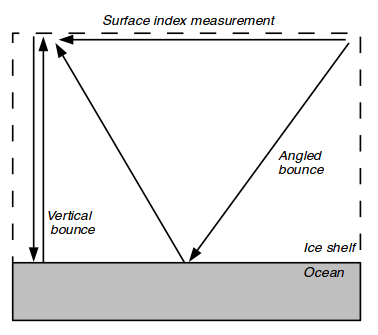
\includegraphics[width=0.6\textwidth]{mooreSetup3.png}
\end{center}
\end{frame}

\begin{frame}{Review of Results from Moore's Bay in 2011-12 Season}
\begin{center}
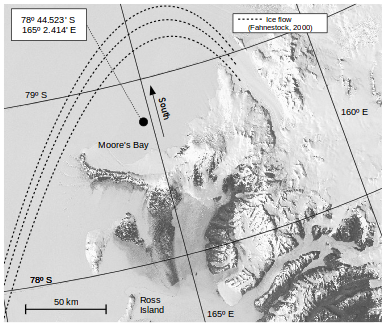
\includegraphics[width=0.6\textwidth]{moore.png}
\end{center}
\end{frame}

\begin{frame}{Review of Results from Moore's Bay in 2011-12 Season}
\begin{center}
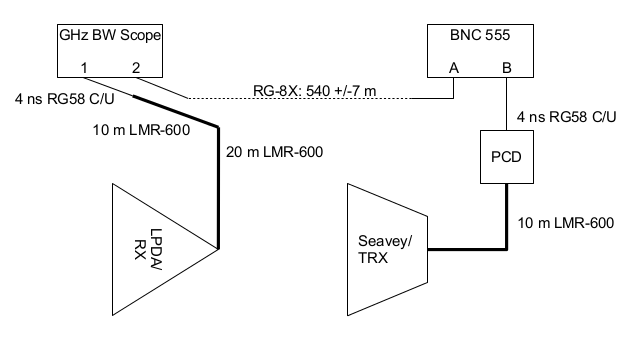
\includegraphics[width=\textwidth]{mooreSetup.png}
\end{center}
\end{frame}

\begin{frame}{Review of Results from Moore's Bay in 2011-12 Season}
\begin{center}
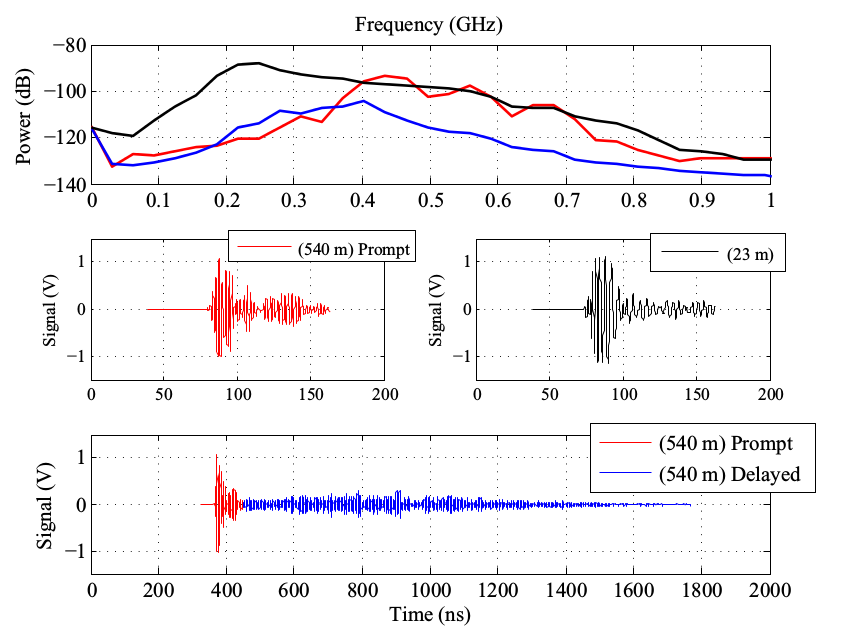
\includegraphics[width=0.85\textwidth]{mooreResult1.png}
\end{center}
\end{frame}

\begin{frame}{Review of Results from Moore's Bay in 2011-12 Season}
\begin{center}
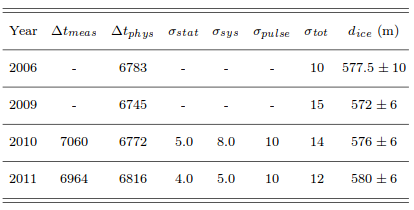
\includegraphics[width=0.75\textwidth]{thicknessMoore.png}
\end{center}
\end{frame}

\begin{frame}{Review of Results from South Pole Station}
\begin{columns}[T]
\begin{column}{0.5\textwidth}
Result from Kravchenko et. al. (2015) builds on prior analyses of surface pulser data by Thomas and others.  The pulser is at the South Pole Station, 4 km away, and the target is the ARA03 array center.  Ray tracing is used to predict the relative timing offsets between antennas and strings.
\end{column}
\begin{column}{0.5\textwidth}
\begin{center}
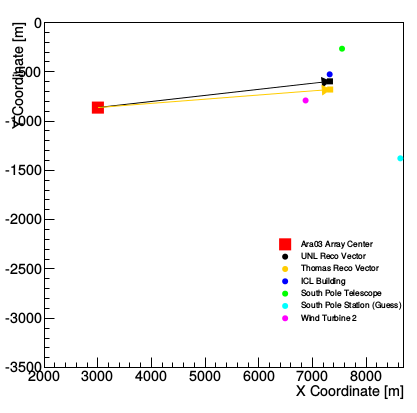
\includegraphics[width=\textwidth]{southpoleSetup.png}
\end{center}
\end{column}
\end{columns}
\end{frame}

\begin{frame}{Review of Results from South Pole Station}
\begin{columns}[T]
\begin{column}{0.5\textwidth}
The following function (now well-motivated) is fit to the data, assuming the asymptotic value of $n=1.78$ for bulk ice at large depths (here increasing $z$ means deeper).
\begin{equation}
n(z) = A-B\exp(-Cz)
\end{equation}
\end{column}
\begin{column}{0.5\textwidth}
\begin{center}
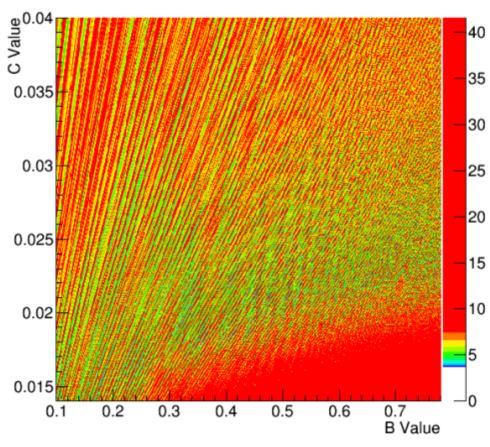
\includegraphics[width=\textwidth]{southpoleSetup2.png}
\end{center}
\end{column}
\end{columns}
\end{frame}

\begin{frame}{Review of Results from South Pole Station}
\begin{columns}[T]
\begin{column}{0.5\textwidth}
Result from Ilya Kravchenko and others (2015) builds on prior analyses of surface pulser data (Gow with $n = 1+k\rho(z)$, Eisen Maud Dronning Core, Schytt theoretical models, RICE data.  \textbf{My question:} This model requires the \textit{assumption} of some model of $n(z)$, and then uses ray-tracing to predict \textit{relative} time-differences between channels. If ray-tracing predicts a different incoming direction than a straight line path, what is that difference in angle?
\end{column}
\begin{column}{0.5\textwidth}
\begin{center}
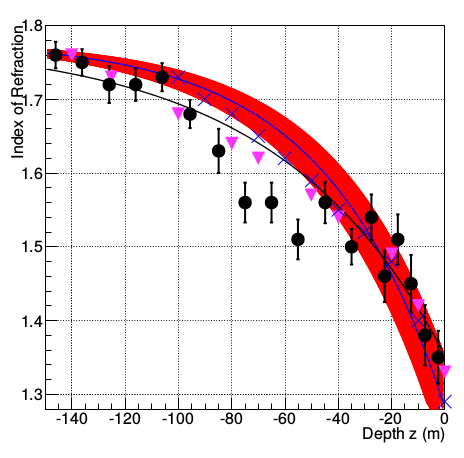
\includegraphics[width=\textwidth]{southpole1.png}
\end{center}
\end{column}
\end{columns}
\end{frame}

\begin{frame}{Review of Results from South Pole Station}
\begin{center}
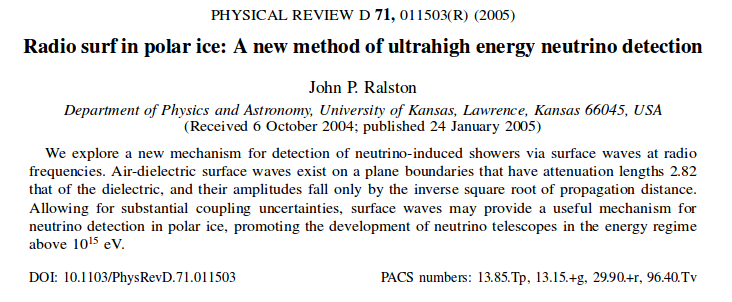
\includegraphics[width=\textwidth]{Ralston.png}
\end{center}
\end{frame}

\begin{frame}{Ten Minute Talk on Ice Shelves and Ice Sheets Near Surface}
\begin{outline}[enumerate]
\1 Dr. Connolly has returned from Weizmann Institute with good news
\1 Part of those discussions require a review of knowledge for ice studies
\2 Emphasis on firn properties
\2 Emphasis on (possible) surface waves
\1 Physics of an ice column
\1 The Landau-Lifshitz/Looyenga equation
\1 Review of Results from Moore's Bay (2011-12)
\1 Review of Results from ARA Analyses (2011-present)
\1 \textbf{Surface Waves}
\end{outline}
\end{frame}

\end{document}